\begin{figure}[t]
	    \begin{center}
		%\fbox{\rule{0pt}{2in} \rule{0.9\linewidth}{0pt}}
   		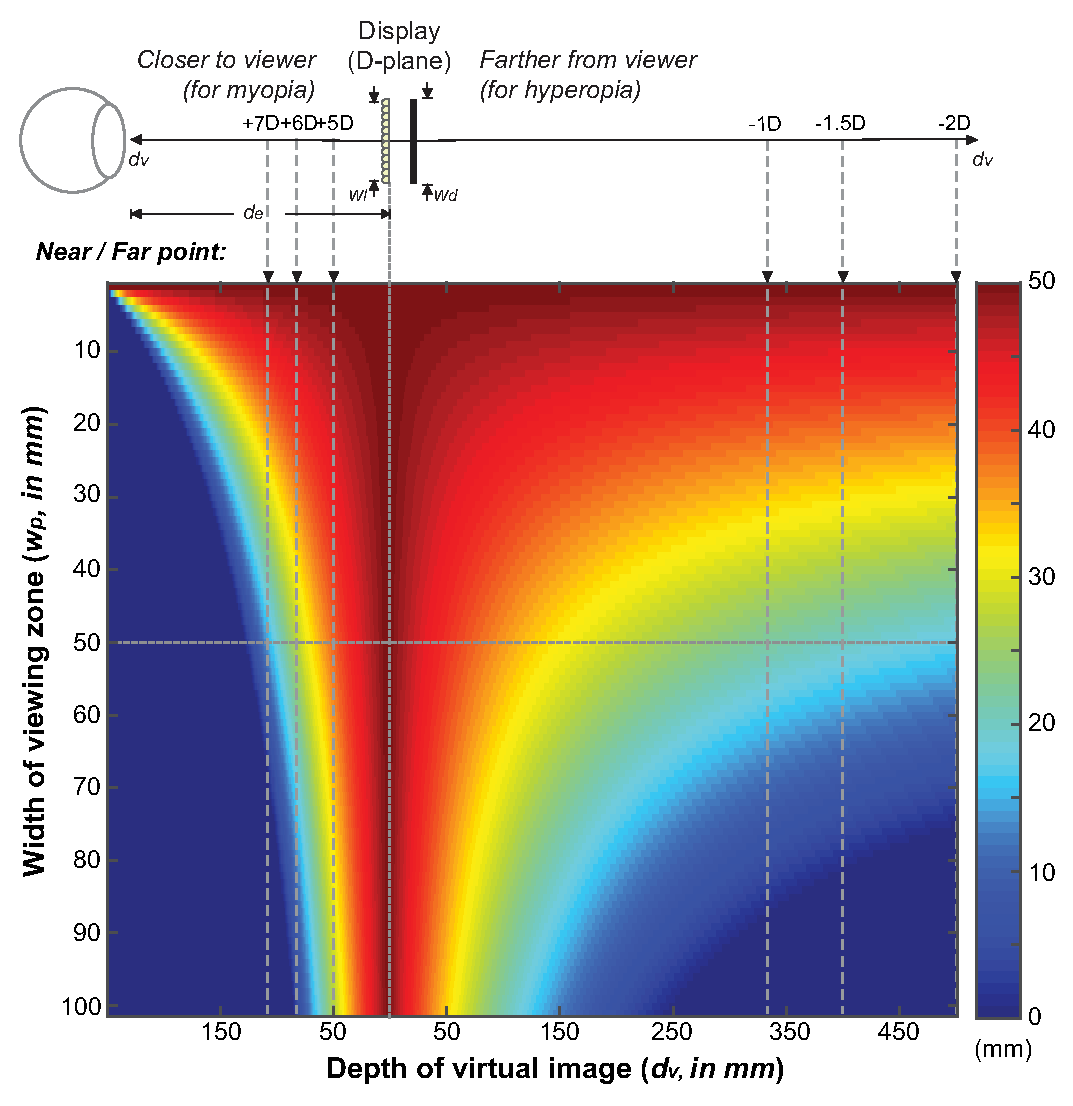
\includegraphics[width=0.90\linewidth]{images/viewingZ_v3.eps}
	    \end{center}
	\caption{(a) The size of perceived virtual image in terms of the width of viewing zone ($w_p$) and the depth of virtual image ($d_v$). Display with the width of display $w_d(=100mm)$ is placed $d_e(=250mm)$ from the viewer.}
\label{fig:viewingZone}
\end{figure}

For the sake of explanation, let us suppose the following viewing environment. As shown in Figure~\ref{fig:viewingZone} (top), a viewer is seeing a 1D display, which has the width $w_l(=50mm)$ and is placed $d_v(=250mm)$ in front of the viewer. 

\subsection{Widths of viewing zone and virtual image}
In Figure~\ref{fig:viewingZone}, the widths of perceived virtual image are shown in terms of two dependent factors: the width of viewing zone ($w_p$) and the depth of virtual image ($d_v$). We also depicted locations of near points (for hyperopia) and far points (for myopia) as dotted vertical line. The maximum size of perceived virtual image is bounded by the size of display ($w_d=50mm$). Note that, optical correction for myopic eyes with $0$ to $+4$ diopter is not required, since the image on display comes to focus on retina without any effect of blurring. With fixed viewing position ($w_p=0$), the size of perceived virtual image is same as the width of display, while the size decreases as more freedom in the viewing point is given. 

\begin{figure}
    \begin{center}
    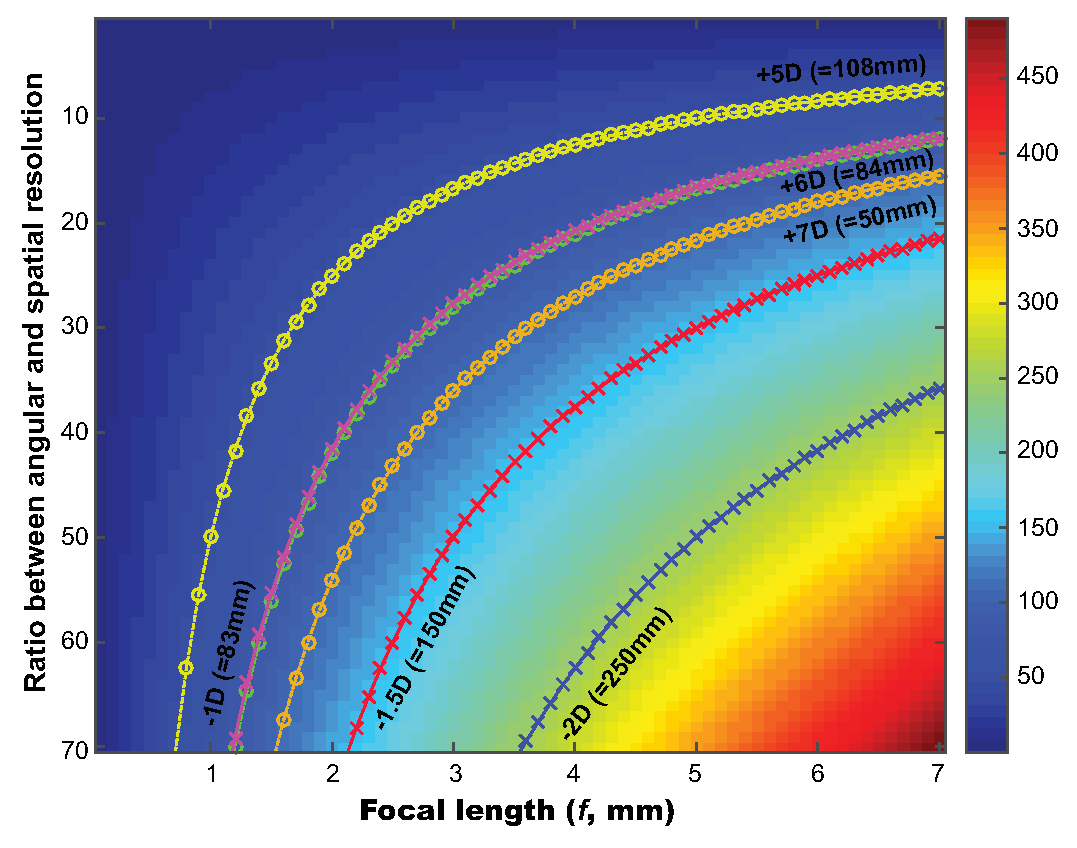
\includegraphics[width=0.95\linewidth]{images/resolutionLimits_v2.eps}
    \end{center}
    \caption{Spatial and Angular resolution limits}
    \label{fig:resolutionLimits}
\end{figure}

\subsection{Spatial and Angular Resolution Limits}
In Figure~\ref{fig:resolutionLimits}, we illustrate the maximum distance at which a virtual image can be placed, maximizing the use of spatial resolution of display based on Equation~\ref{eq:resolutionLimits}. We draw the figure in terms of two parameters: the ratio between angular and spatial resolution ($=\Delta t / \Delta v$) and the focal length ($f$). As expected, as both parameters increase, a farther virtual image can be rendered. Each line in the figure represents the minimum required system setting for correcting eye-aberration (\ie, +5D to +7D for myopia, -1D to -2D for hyperopia).

\subsection{Eye Correction limits}
According to the anti-aliasing display analysis by Zwicker\etal~\cite{zwicker2006antialiasing}, given a display with spatial sample spacing of $\Delta t$ and angular sample spacing $\Delta v$, the maximum plane depth where the scene can be represented with full spatial resolution of the display is $|z| = \Delta t / \Delta v$, where $z$ is the distance between the focal plane and the display. As there is a one-to-one mapping between depth of focal plane and eye aberration (in diopter D, given in mm), this depth limit sets a constraint on the correction power of a display with a fixed spatial and angular resolution. The limitation of eye aberration that can be corrected by a display with $\Delta t$ and $\Delta v$ is:
$$D = \frac{1000}{d_e-\Delta t / \Delta v}$$
where $d_e$ is the distance between viewer and display. More intuitively, for the screen size of an iPhone 6s (120 mm diagonal) and a normal viewing distance of 250 mm, in order to correct a myopic eye with -2D aberration, we require a the virtual image plane to be placed 200 mm behind (away from the viewer) the display.

\subsection{Higher order aberration} \label{ss:Higherorderaberration}
Any type of viewing-independent vision-correcting display that supports free eye-movement would create error in correcting higher-order aberration, which includes coma, astigmatism, distortion, and spherical aberration. To prove it, suppose that $N$ parallel light rays $l_i$ ($i=1,2,...,N$) is coming from the virtual plane to the eye's pupil plane, and each ray is uniformly spaced by $\Delta h$, which is sufficiently smaller than the size of eye's entrance pupil. Given any types of aberration, light rays entering eye's entrance pupil would create transverse error $\epsilon_i$. Now, let us assume the eye is moving in lateral direction with an amount larger than $\Delta h$. If there appears a non-linear variation in transverse error difference (\ie, $|\epsilon_i -\epsilon_{i-1}|$), light fields should be recalculated based on the position of eye for accurate correction. Unlike low-order aberrations (\ie, myopia and hyperopia) that produce a constant transverse error difference between neighboring light rays, higher-order aberrations have transverse error that would vary periodically (see supplemental material for more details). This introduces difficulties to make the viewing-independent vision-correcting display for higher-order aberration. In Figure~\ref{fig:rayspace_highorderaberration}, we illustrate ray space diagram for 4 major types of high-order aberration: coma, astigmatism, distortion, and spherical aberration. 

